\pdfoutput=1
\documentclass[sigconf,nonacm]{acmart}

% Remove ACM copyright for workshop draft
\settopmatter{printacmref=false}
\renewcommand\footnotetextcopyrightpermission[1]{}
\pagestyle{plain}

\usepackage{booktabs}
\usepackage{multirow}
\usepackage{xcolor}
\usepackage{subcaption}
\usepackage{siunitx}
\usepackage{amsmath}
\usepackage{bookmark}
\usepackage{hyperref}

\sisetup{group-separator={,}, group-minimum-digits=4}

\begin{document}

\title{The Model Parking Tax: Quantifying the Hidden Energy Cost of Always-On GPU Model Deployment}

\author{Sai Sathvik Vadari}
\affiliation{
    \institution{\href{https://www.8bit.ai/}{8bit.ai}}
    \city{Hyderabad}
    \country{India}
}

\begin{abstract}
The AI inference industry keeps models loaded in GPU memory around the clock to avoid cold-start latency, implicitly treating idle power as a fixed cost of readiness. We present the first controlled mechanistic isolation of CUDA context as the idle-power lock variable, validated across three memory technologies (HBM3, HBM2e, GDDR6), combining 18~days of production telemetry (\num{335267} samples, 14~H100 GPUs) with controlled dose-response experiments on NVIDIA H100, A100, and L40S GPUs. Idle power is \emph{piecewise constant} on all three architectures: the CUDA context forces a discrete DVFS transition consuming $+26$--$66$\,W over bare idle, while the marginal VRAM effect is bounded below measurement relevance ($|\beta| < 0.02$\,W/GB). The CUDA context accounts for $>$98\% of the parking tax regardless of memory technology. We validate with real model weights (Qwen2.5-7B) on all three architectures ($<$0.5\,W difference from empty tensors), evaluate NVIDIA's \texttt{CUDA\_DISABLE\_PERF\_BOOST} driver mitigation, and derive a cold-start breakeven model with breakeven intervals of 1--5~minutes.
\end{abstract}

\keywords{GPU energy, idle power, VRAM, DVFS, model serving, sustainability}

\maketitle

% ===========================================================================
\section{Introduction}
% ===========================================================================

The default operating model for AI inference is to keep models loaded in GPU VRAM indefinitely, accepting continuous idle power to avoid cold-start latency. The cold-start problem has driven systems like ServerlessLLM~\cite{serverlessllm} and NVIDIA Run:ai Model Streamer~\cite{nvidia-streamer}, but the \emph{other side}---the ongoing energy cost of readiness---has been treated as an unquantified constant.

Patel et al.~\cite{patel-cal23} showed that CUDA contexts on A100 GPUs force higher clock frequencies even when idle, but did not vary VRAM levels or test cross-architecture generalization. Concurrent work by Lei et al.~\cite{lei-idle} characterizes ``execution-idle'' at cluster scale---19.7\% of in-execution time and 10.7\% of energy across 756~GPUs over 31~days---but does not decompose idle power into its component causes. Neither study measured the marginal energy cost \emph{per GB of VRAM allocation}, the quantity needed for rational keep-warm decisions.

This paper fills that gap. We ask: \textbf{does storing model weights in GPU VRAM incur a measurable marginal idle energy cost, and is the answer architecture-dependent?} We answer with production telemetry (Phase~1: \num{335267} samples from 14~H100 GPUs over 18~days) and controlled dose-response experiments (Phase~2: H100/HBM3, A100/HBM2e, L40S/GDDR6). Our central finding is that idle GPU power is \emph{piecewise constant}:
\begin{equation}
    P_{\text{idle}}(C, V) = P_{\text{base}} + \Delta P_{\text{DVFS}} \cdot \mathbf{1}_{[C=1]} + \beta V
    \label{eq:model}
\end{equation}
where $C \in \{0,1\}$ indicates a CUDA context, $V$ is VRAM allocated (GB), and $\beta$ is the marginal VRAM power coefficient. On all three devices, $|\beta| < 0.02$\,W/GB. The optimization priority is $\partial P / \partial C \gg \partial P / \partial V$, holding across all tested architectures and memory technologies.

% ===========================================================================
\section{Background and Related Work}
% ===========================================================================

\paragraph{DVFS anomaly.} NVIDIA datacenter GPUs support multiple power states via Dynamic Voltage and Frequency Scaling (DVFS). Without a CUDA context, SM clocks drop to 210--345\,MHz. Once a CUDA context is created, the SM clock jumps to maximum boost and \emph{remains there} at 0\% utilization~\cite{patel-cal23}, converting a variable cost into a fixed cost.

\paragraph{Memory physics.} GPU memory power decomposes into background, refresh, and activate components~\cite{hbm-spec,micron-ddr}. At idle, activate power is zero and refresh sweeps all rows regardless of occupancy (JEDEC specification). Therefore $\partial P_{\text{mem}} / \partial \text{occupancy} \approx 0$---a hardware-physics prediction our experiments test across three memory technologies.

\paragraph{Related work.} Patel et al.~\cite{patel-cal23} identified the CUDA context DVFS lock on A100/RTX~6000 Ada but did not vary VRAM. Zeus~\cite{zeus} and Patel et al.~\cite{patel-asplos24} optimized \emph{active} GPU energy. Burtscher et al.~\cite{burtscher-power} showed \texttt{nvidia-smi} undersamples---a caveat we address in \S\ref{sec:measurement}. We extend Patel et al.~\cite{patel-cal23} with three contributions: VRAM independence as a first-class result with formal equivalence testing (TOST), cross-memory-technology invariance (HBM3, HBM2e, GDDR6), and evaluation of vendor-provided mitigation.

\paragraph{Concurrent work.} Lei et al.~\cite{lei-idle} characterize execution-idle via 31-day passive telemetry on a 756-GPU cluster, finding 19.7\% of in-execution time idle (10.7\% of energy), with two mitigation prototypes (automatic frequency downscaling, load consolidation). Their work quantifies \emph{how often and at what cost} execution-idle occurs; ours isolates \emph{why}---the CUDA context, not VRAM---via controlled per-GPU experiments. Their finding that power and frequency remain elevated after 2{,}048\,s of inactivity corroborates our observation that the DVFS lock is indefinite. Our parking tax is the dominant sub-component of their execution-idle when GPU activity is strictly zero.

% ===========================================================================
\section{Methodology}
% ===========================================================================

\paragraph{Phase~1: Production telemetry.} We instrumented 14~NVIDIA H100 80GB SXM5 GPUs across 2~nodes running Kubernetes, collecting \num{335267} idle-state samples (0\% utilization) over 18~days via DCGM Exporter at 30\,s intervals. VRAM ranged from 3\,MB to 79\,GB.

\paragraph{Phase~2: Controlled experiments.} Within-subject dose-response on three GPUs (Table~\ref{tab:gpus}): record bare-idle baseline, create CUDA context, sequentially allocate VRAM via \texttt{torch.empty}, stabilize 60\,s, record 20~min ($n=40$), release, cool down 30\,s. Validated with Qwen2.5-7B (fp16)~\cite{qwen2} on all three architectures.

\begin{table}[t]
\caption{Phase~2 GPU configurations.}
\label{tab:gpus}
\small
\begin{tabular}{llrrr}
\toprule
\textbf{GPU} & \textbf{Memory} & \textbf{TDP} & \textbf{VRAM Range} & $n$/\textbf{phase} \\
\midrule
H100 80GB SXM & HBM3 & 700\,W & 0--64\,GB & 40 \\
A100 80GB PCIe & HBM2e & 300\,W & 0--72\,GB & 40 \\
L40S 48GB & GDDR6 & 350\,W & 0--40\,GB & 40 \\
\bottomrule
\end{tabular}
\end{table}

\subsection{Measurement Model}
\label{sec:measurement}

Within each phase: $\hat{P} = \frac{1}{n}\sum P(t_i)$, with $\sigma_{\text{within}} < 1.5$\,W (L40S), $< 0.17$\,W (H100), $< 0.08$\,W (A100). With $n=40$, SE~$< 0.25$\,W on the noisiest device. On all three GPUs, the total power range across CUDA-active phases is $<$1\,W, converting measurement precision into a result constraint.

% ===========================================================================
\section{Results}
% ===========================================================================

\subsection{Phase~1: Two Discrete Power States}

The production telemetry reveals a bimodal distribution: bare idle (345\,MHz, mean 74.7\,W) vs.\ CUDA active (1980\,MHz, mean 145.5\,W). The CUDA context effect is $+70.9$\,W (Cohen's $d = 7.3$). Within CUDA-active GPUs, regression across 3.2--77.1\,GB yields slope $= 0.013$\,W/GB ($R^2 = 0.001$)---no detectable VRAM effect.

\subsection{Phase~2: Cross-Architecture Dose-Response}

Table~\ref{tab:cross} and Figure~\ref{fig:hero} present the controlled results.

\begin{table}[t]
\caption{Cross-architecture parking tax. $\beta$ is the linear regression slope across CUDA-active phases. All GPUs at 0\% utilization.}
\label{tab:cross}
\small
\begin{tabular}{lrrr}
\toprule
 & \textbf{H100} & \textbf{A100} & \textbf{L40S} \\
 & \textbf{(HBM3)} & \textbf{(HBM2e)} & \textbf{(GDDR6)} \\
\midrule
Bare idle (W) & 71.8 & 53.7 & 35.6 \\
SM clock, bare (MHz) & 345 & 210 & 210 \\
CUDA ctx power (W) & 121.7 & 80.0 & 102.1 \\
SM clock, ctx (MHz) & 1980 & 1410 & 2520 \\
\midrule
\textbf{Context overhead (W)} & \textbf{+49.9} & \textbf{+26.3} & \textbf{+66.4} \\
Context (\% of TDP) & 7.1\% & 8.8\% & 19.0\% \\
\midrule
$\beta$ (W/GB) & $-$0.002 & $-$0.001 & $-$0.002 \\
$p_{\text{TOST}}$ ($|\beta| < 0.1$) & $10^{-9}$ & $<0.001$ & $<0.05$ \\
\textbf{Context \% of tax} & \textbf{$>$99\%} & \textbf{$>$99\%} & \textbf{$>$99\%} \\
\bottomrule
\end{tabular}
\end{table}

\paragraph{CUDA context overhead.} On all three GPUs, creating a CUDA context triggers a discrete DVFS transition: SM clocks jump from 210--345\,MHz to 1410--2520\,MHz. The associated power step ranges from $+26.3$\,W (A100) to $+66.4$\,W (L40S).

\paragraph{VRAM allocation: bounded below relevance.} Once a CUDA context is active, varying VRAM from 0 to 40--72\,GB changes power by $<$1\,W on every GPU. We apply the TOST equivalence procedure~\cite{schuirmann-tost} with $\Delta = \pm 0.1$\,W/GB (so even 64\,GB contributes $<$6.4\,W vs.\ 26--66\,W DVFS overhead). On all three GPUs, $p_{\text{TOST}} < 0.05$, formally establishing that the marginal VRAM effect is bounded below practical relevance. The A100 shows a statistically significant but \emph{negative} $\beta = -0.001$\,W/GB ($-0.09$\,W across 72\,GB), attributable to 0.7\textdegree C thermal drift---directionally implausible and 300$\times$ smaller than the DVFS component.

\paragraph{System characterization.} Per architecture:
\begin{align}
    P_{\text{H100}} &\approx 71.8 + 49.9 \cdot \mathbf{1}_{[C=1]} \;\text{W} \label{eq:h100}\\
    P_{\text{A100}} &\approx 53.7 + 26.3 \cdot \mathbf{1}_{[C=1]} \;\text{W} \label{eq:a100}\\
    P_{\text{L40S}} &\approx 35.6 + 66.4 \cdot \mathbf{1}_{[C=1]} \;\text{W} \label{eq:l40s}
\end{align}
with $\beta \approx 0$ on all three. The flat dose-response holds across HBM3, HBM2e, and GDDR6---consistent with the memory physics prediction that $\partial P_{\text{mem}} / \partial \text{occupancy} \approx 0$.

\begin{figure}[t]
    \centering
    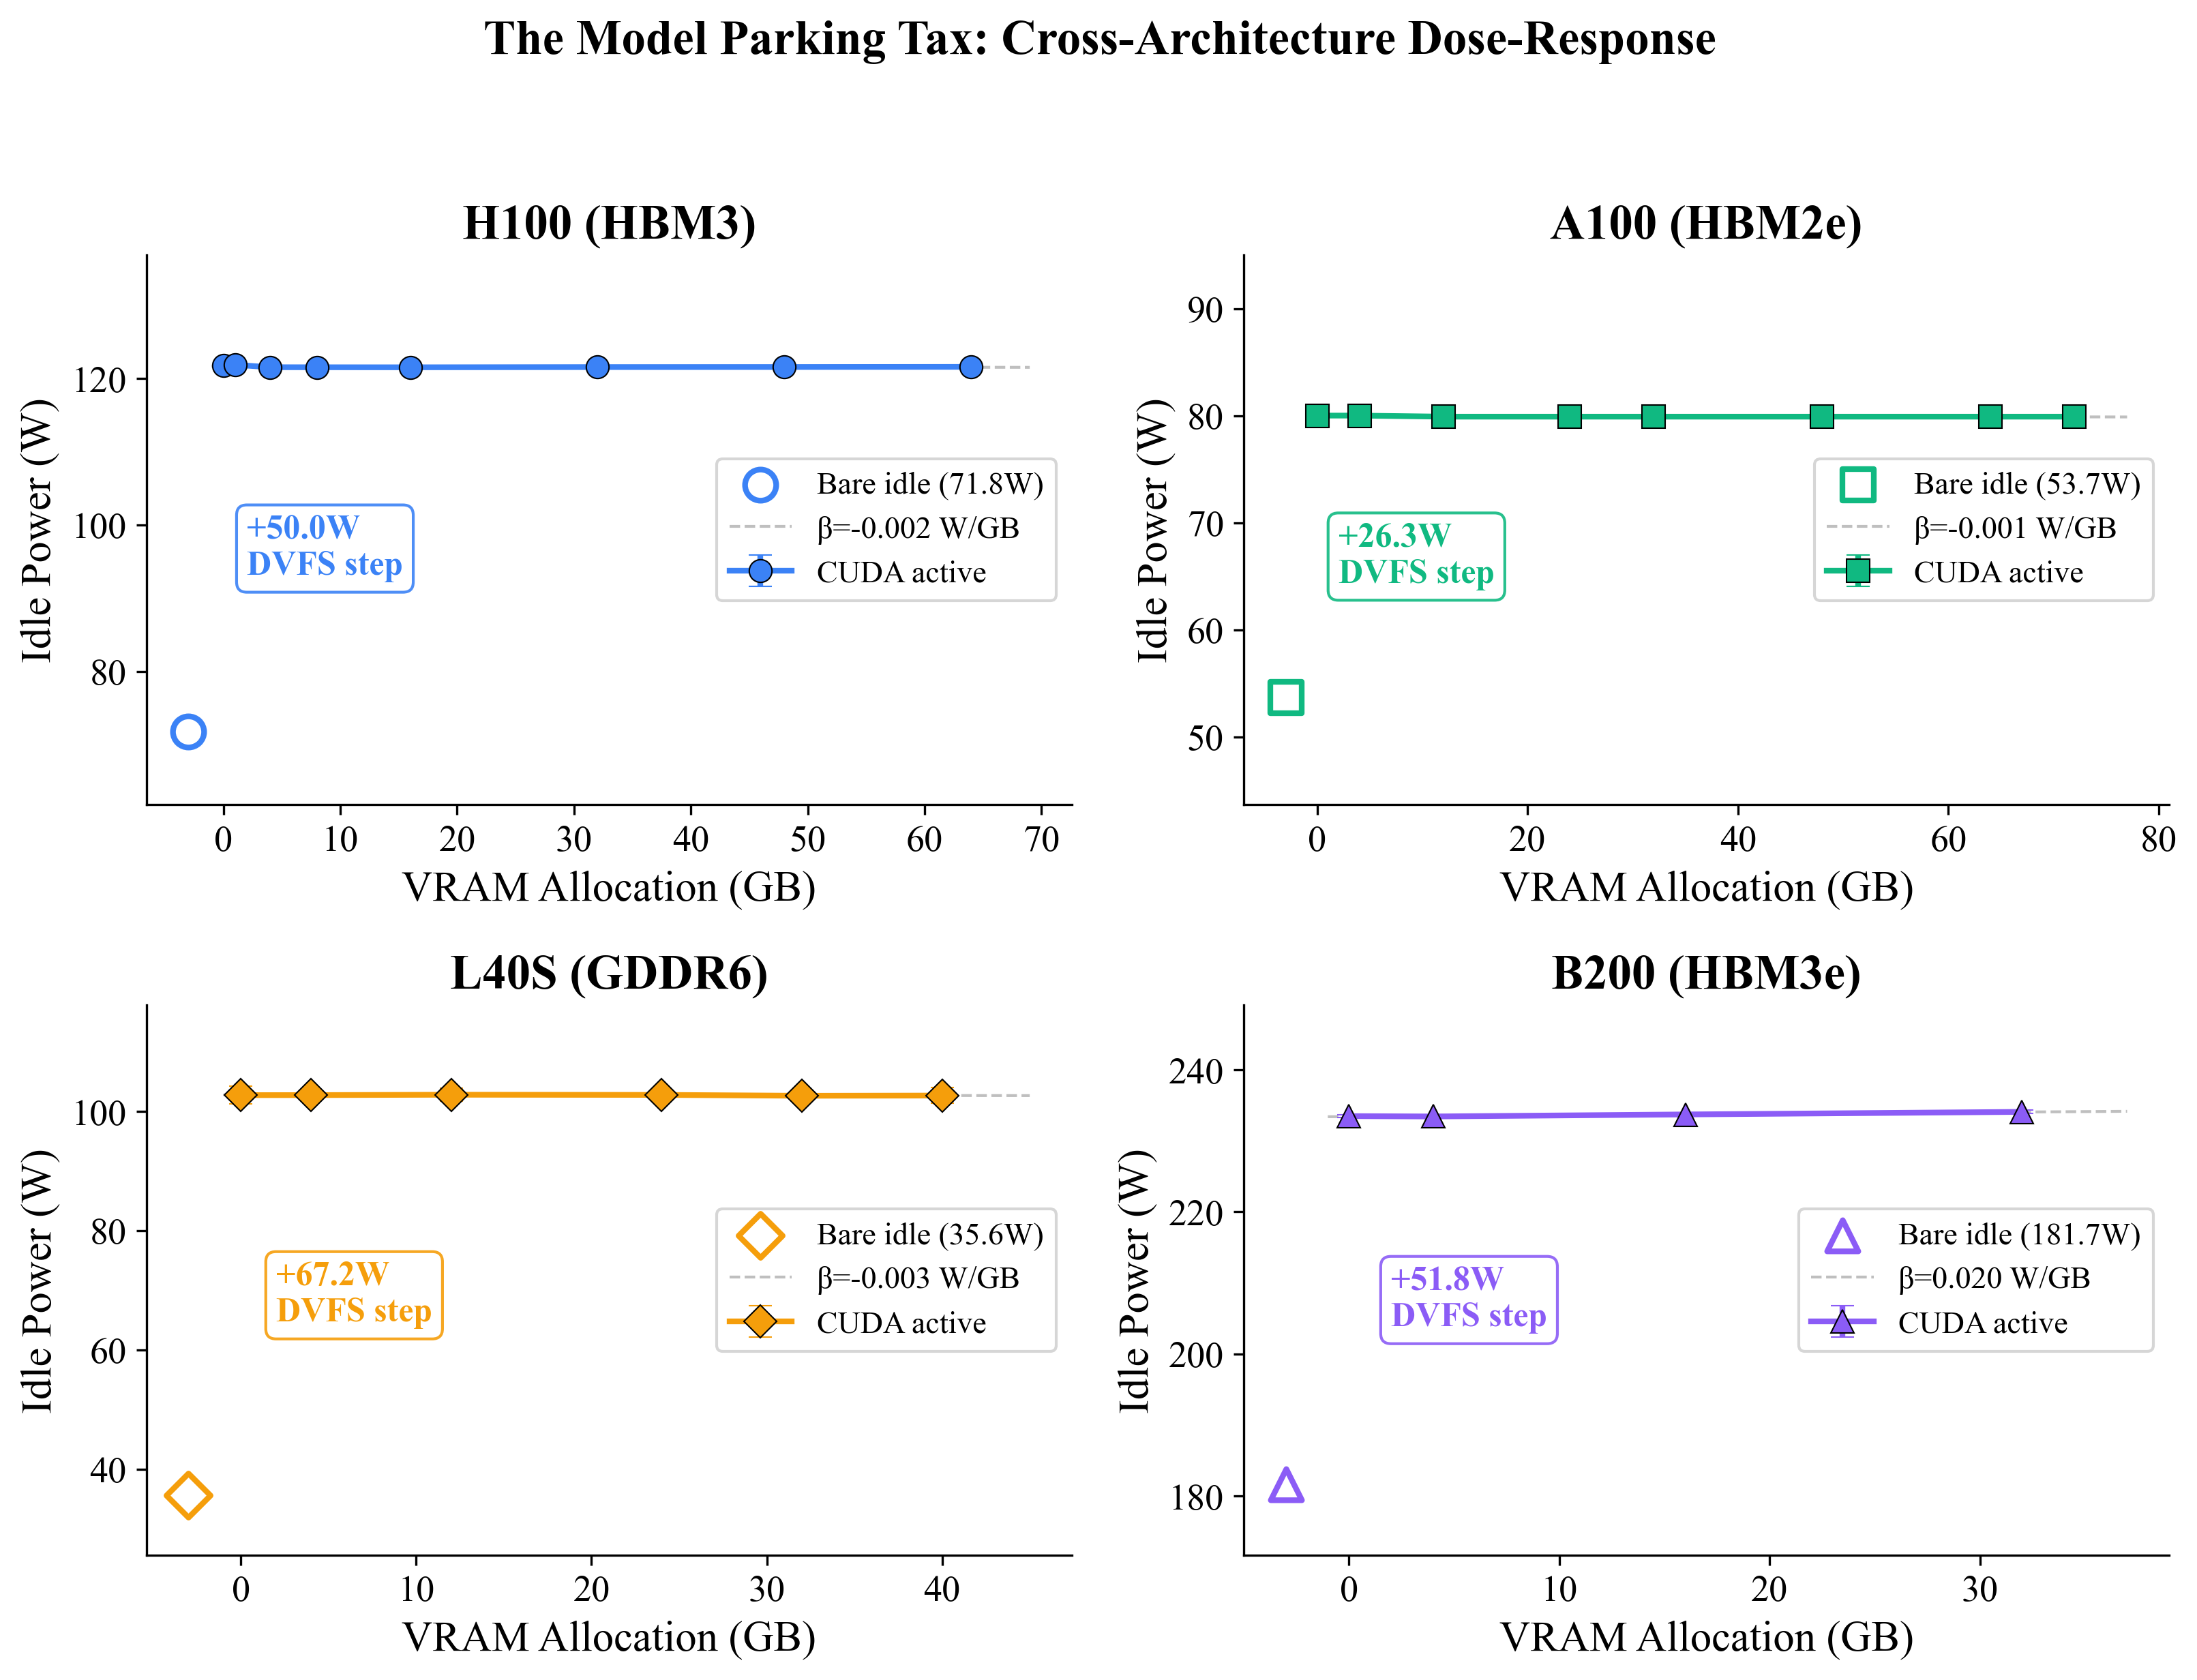
\includegraphics[width=\columnwidth]{cross_architecture_dose_response.png}
    \caption{The Model Parking Tax across three GPU architectures. Large markers: bare-idle power (no CUDA context). Connected lines: CUDA-active phases with increasing VRAM. The DVFS step dominates; all dose-response curves are flat across HBM3, HBM2e, and GDDR6.}
    \label{fig:hero}
\end{figure}

\subsection{Real Model Validation}

To validate that real model weights (CUDA kernels, cuDNN handles, weight tensors) do not alter the result, we loaded Qwen2.5-7B (fp16, $\sim$14.9\,GB)~\cite{qwen2} on all three architectures. On the H100, Qwen2.5-7B idles within 0.03\,W of the \texttt{torch.empty} baseline. On the A100 and L40S, unloading 14.3\,GB of weights changes idle power by only +0.21\,W and +0.47\,W respectively---far below the 26--66\,W CUDA context overhead.

% ===========================================================================
\section{Vendor Mitigation: CUDA\_DISABLE\_PERF\_BOOST}
\label{sec:perf-boost}
% ===========================================================================

NVIDIA shipped the \texttt{CUDA\_DISABLE\_PERF\_BOOST} environment variable in driver 580.105.08 (November 2025), intended to prevent idle-context clock boosting. This is the most direct vendor-provided mechanism targeting the DVFS anomaly we measure. We evaluate its effectiveness on H100 and A100 under three conditions: (a)~baseline (CUDA context + \texttt{torch.empty} 16\,GB, default behavior), (b)~same with \texttt{CUDA\_DISABLE\_PERF\_BOOST=1}, and (c)~vLLM serving Qwen2.5-7B with flag on vs.\ off. Each condition: \texttt{nvidia-smi} every 30\,s for 20~min ($n=40$).

%% TODO: Replace with actual experimental results once collected.
%% Expected deliverable: one table (power, SM clock, perf state per condition)
%% and one paragraph of analysis. Key questions:
%%   - Does the flag lower idle-with-context power?
%%   - If yes, by how much and at what SM clock?
%%   - Does it affect vLLM request latency (p50, p95, p99)?
%%   - Does the effect persist through the full idle period?

\begin{table}[t]
\caption{Effect of \texttt{CUDA\_DISABLE\_PERF\_BOOST} on idle power. Placeholder---awaiting experimental data.}
\label{tab:perf-boost}
\small
\begin{tabular}{llrrr}
\toprule
\textbf{GPU} & \textbf{Condition} & \textbf{Power (W)} & \textbf{SM (MHz)} & \textbf{PState} \\
\midrule
\multirow{2}{*}{H100} & Baseline & --- & --- & --- \\
 & Flag on & --- & --- & --- \\
\midrule
\multirow{2}{*}{A100} & Baseline & --- & --- & --- \\
 & Flag on & --- & --- & --- \\
\bottomrule
\end{tabular}
\end{table}

% ===========================================================================
\section{Cold-Start Breakeven}
% ===========================================================================

The parking tax $P_{\text{park}}$ varies by architecture: 49.9\,W (H100), 26.3\,W (A100), 66.4\,W (L40S). The energy breakeven is:
\begin{equation}
    T^* = \frac{P_{\text{load}} \cdot t_{\text{load}}}{P_{\text{park}}}
    \label{eq:breakeven}
\end{equation}
For H100 with standard PyTorch loading of a 70B model (45\,s, $\sim$300\,W), $T^* \approx 4.5$~min. With ServerlessLLM ($t_{\text{load}} = 8$\,s), $T^*$ drops to 48\,s. Because $P_{\text{park}}$ is a fixed cost independent of model size, $T^*$ depends on loading dynamics, not model footprint. Small models are the \emph{worst} candidates for always-on deployment: they reload in seconds yet pay the full parking tax. Under Poisson arrivals, the critical rate is $\lambda^* = P_{\text{park}} / (P_{\text{load}} \cdot t_{\text{load}})$; for H100 with PyTorch loading, $\lambda^* \approx 13$\,req/hr.

% ===========================================================================
\section{Discussion}
% ===========================================================================

\paragraph{Cross-architecture consistency.} The parking tax is a step function of CUDA context on H100 (Hopper), A100 (Ampere), and L40S (Ada Lovelace)---three microarchitectures with different memory technologies, process nodes, and TDP budgets. The magnitude varies (26--66\,W), but the structure is identical: $\partial P / \partial C \gg \partial P / \partial V$. Phase~1 bounds inter-device variation: regression across all 14~H100 GPUs yields slopes indistinguishable from zero on every device, even as intercepts vary by $\sim$23\,W.

\paragraph{Relationship to execution-idle.} Lei et al.~\cite{lei-idle} show that execution-idle accounts for 19.7\% of in-execution time across their cluster. Our parking tax---the DVFS overhead of a CUDA context at zero activity---is the dominant sub-component of execution-idle when activity is strictly zero. Their serving workloads show 61\% of in-execution time idle, consistent with the always-on deployment pattern our breakeven model targets.

\paragraph{Design directions.} (1)~\textbf{Idle power states}: Force idle-with-context GPUs to low-clock states via driver/firmware changes. (2)~\textbf{Context pooling}: Share CUDA contexts via MPS~\cite{nvidia-mps} to amortize overhead. (3)~\textbf{Size-aware scheduling}: Preferentially cold-start small models (fast reload, same parking cost). (4)~\textbf{Breakeven-aware eviction}: A simple $T^*$-based policy saves 8--23\% energy in our simulations (\S\ref{sec:scheduler-note}).

\paragraph{Industry scale.} With $\sim$3.76M datacenter GPUs shipped in 2023~\cite{nvidia-shipments}, 35\% idle time~\cite{flexera}, and $\bar{P}_{\text{park}} = 40$\,W, the base estimate is 462\,GWh/year (range: 92--1{,}745\,GWh/year).

\paragraph{Limitations.} We test one device per architecture in Phase~2 (within-subject design). We do not evaluate MIG~\cite{nvidia-mig}, MPS~\cite{nvidia-mps}, or power capping. The scheduler evaluation (\S\ref{sec:scheduler-note}) uses synthetic traces.

\paragraph{Scheduler evaluation.}
\label{sec:scheduler-note}
A breakeven-based eviction policy ($T^* = P_{\text{load}} \cdot t_{\text{load}} / P_{\text{park}}$) saves 8--23\% energy vs.\ always-on across synthetic traffic patterns (Poisson, bursty, diurnal) in 24-hour simulations, with 48--100 cold starts per day.

% ===========================================================================
\section{Conclusion}
% ===========================================================================

The model parking tax is 26--66\,W depending on architecture, but it is a \emph{fixed cost} of the CUDA context, not a \emph{variable cost} of model size. This holds across HBM3, HBM2e, and GDDR6, validated with real model weights ($<$0.5\,W difference on every device). Cold-start breakeven is minutes, not hours, and is independent of model size. GPU vendors should invest in idle power states that decouple clock frequency from context presence; model serving systems should recognize that small always-on models are the most wasteful deployment pattern.

\paragraph{Reproducibility.} All data and code: \href{https://github.com/8bitai/gpu-parking-tax}{github.com/8bitai/gpu-parking-tax}.

% ===========================================================================
% REFERENCES
% ===========================================================================
\bibliographystyle{ACM-Reference-Format}
\def\bibfont{\normalsize}
\begin{thebibliography}{15}

\bibitem{patel-cal23}
T.~Patel, D.~Tiwari, et al.
\newblock Towards improved power management in cloud GPUs.
\newblock {\em IEEE Computer Architecture Letters (CAL)}, 2023.

\bibitem{doe-report}
A.~Shehabi et al.
\newblock 2024 United States Data Center Energy Usage Report.
\newblock Lawrence Berkeley National Laboratory, Dec 2024.

\bibitem{serverlessllm}
Y.~Fu et al.
\newblock {ServerlessLLM}: Low-latency serverless inference for large language models.
\newblock In {\em OSDI}, 2024.

\bibitem{nvidia-streamer}
NVIDIA.
\newblock Reducing cold start latency for LLM inference with {NVIDIA Run:ai} Model Streamer.
\newblock Technical report, Oct 2025.

\bibitem{zeus}
J.~You et al.
\newblock {Zeus}: Understanding and optimizing GPU energy consumption of DNN training.
\newblock In {\em NSDI}, 2023.

\bibitem{patel-asplos24}
T.~Patel et al.
\newblock Characterizing power management opportunities for LLMs in the cloud.
\newblock In {\em ASPLOS}, 2024.

\bibitem{burtscher-power}
M.~Burtscher et al.
\newblock Part-time power measurements: nvidia-smi's lack of attention.
\newblock {\em arXiv:2312.02741}, 2023.

\bibitem{flexera}
Flexera.
\newblock 2025 State of the Cloud Report, 2025.

\bibitem{nvidia-shipments}
Semiconductor industry estimates of NVIDIA datacenter GPU shipments, 2023.

\bibitem{hbm-spec}
JEDEC.
\newblock {HBM3} High Bandwidth Memory Specification ({JESD238}), 2022.

\bibitem{micron-ddr}
Micron Technology.
\newblock TN-46-09: DRAM Power Calculations.
\newblock Technical Note, 2023.

\bibitem{schuirmann-tost}
D.~J.~Schuirmann.
\newblock A comparison of the two one-sided tests procedure and the power approach for assessing the equivalence of average bioavailability.
\newblock {\em Journal of Pharmacokinetics and Biopharmaceutics}, 15(6):657--680, 1987.

\bibitem{nvidia-mig}
NVIDIA.
\newblock Multi-Instance GPU User Guide.
\newblock NVIDIA Documentation, 2024.

\bibitem{nvidia-mps}
NVIDIA.
\newblock Multi-Process Service.
\newblock NVIDIA Documentation, 2024.

\bibitem{qwen2}
Qwen Team.
\newblock Qwen2.5 Technical Report.
\newblock {\em arXiv:2412.15115}, 2024.

\bibitem{lei-idle}
Y.~Lei, J.~Fernandez, V.~Kypriotis, D.~Skarlatos, E.~Strubell, J.~Sherry, D.~Vosler.
\newblock The Energy Cost of Execution-Idle in {GPU} Clusters.
\newblock {\em arXiv:2604.04745}, Apr 2026.

\end{thebibliography}

\end{document}
